\documentclass[a4paper,10pt]{article}

\usepackage{amsmath}
\usepackage[utf8]{inputenc}
\usepackage{geometry}
\usepackage[document]{ragged2e}
\usepackage{graphicx}
\usepackage{enumerate}

\geometry{left=2.5cm,right=2.5cm,top=3cm,bottom=3cm}
\parindent0mm

\renewcommand{\baselinestretch}{1.5}
\renewcommand{\theenumi}{\alph{enumi}}

\title{ICG · Übung 4}
\author{Benjamin Schmidt}
\date{\today}

\begin{document}
	\maketitle

	\section*{Aufgabe 1}

	\begin{figure}[htb]
		\centering
		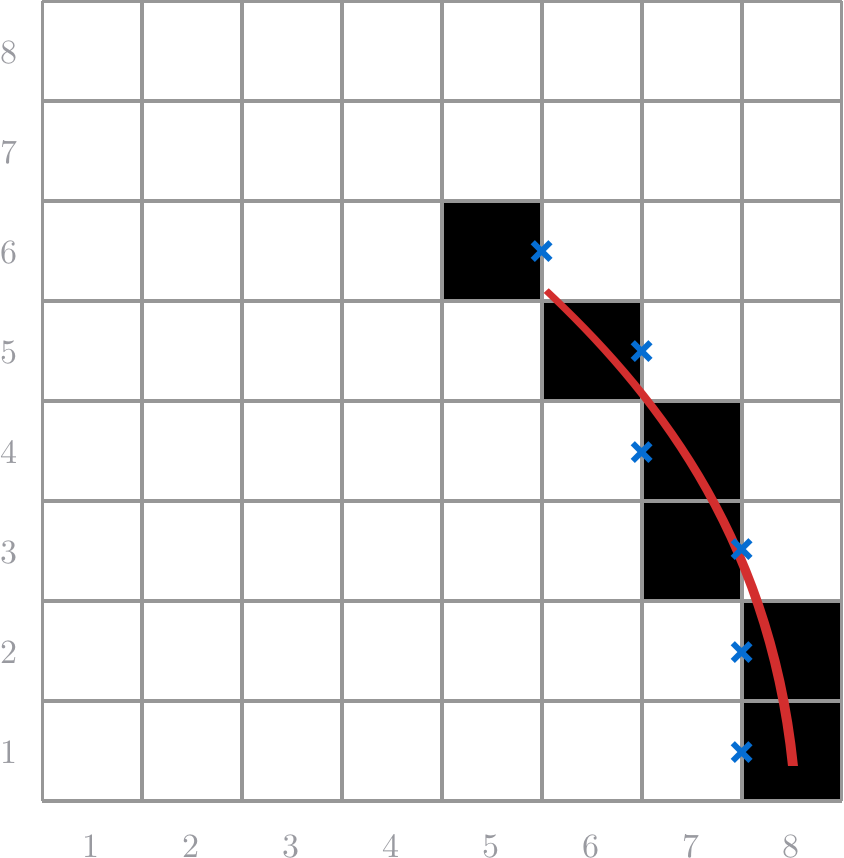
\includegraphics[scale=0.25]{Grid.png}
	\end{figure}

	\textbf{Rechnungen:} \\
	Im ersten Oktanten gilt $F(x - 0.5, y + 1)$, also gilt: \\
	$F(x,y) = x^2 + y^2 - r^2 = (x - 0.5)^2 + (y + 1)^2 - 64$ (für $r = 8$).\\~\\

	Startpunkt ist $(8, 0)$, Midpoint wird gewählt als $(x - 0.5, y + 1)$ also $(7.5, 1)$. \\
	Auszufüllendes Kästchen vom Midpoint aus gesehen ist mit Pfeilen jeweilig markiert.

	\begin{enumerate}[1.]
		\item $F(8,0) = (8 - 0.5)^2 + (0 + 1)^2 - 64 = -6.75 \leq 0$   ($\rightarrow$)
		\item $F(8,1) = (8 - 0.5)^2 + (1 + 1)^2 - 64 = -3.75 \leq 0$   ($\rightarrow$)
		\item $F(8,2) = (8 - 0.5)^2 + (2 + 1)^2 - 64 = 1.25 \geq 0$     ($\leftarrow$)
		\item $F(7,3) = (7 - 0.5)^2 + (3 + 1)^2 - 64 = -5.75 \leq 0$   ($\rightarrow$)
		\item $F(7,4) = (7 - 0.5)^2 + (4 + 1)^2 - 64 = 3.25 \geq 0$     ($\leftarrow$)
		\item $F(6,5) = (6 - 0.5)^2 + (5 + 1)^2 - 64 = 2.25 \geq 0$     ($\leftarrow$)
	\end{enumerate}

	\section*{Aufgabe 2}

	\begin{enumerate}[(I)]
		\item $F(x - 0.5, y + 1)$
		\item $F(x - 1, y + 0.5)$
		\item $F(x - 1, y - 0.5)$
		\item $F(x - 0.5, y - 1)$
		\item $F(x + 0.5, y + 1)$
		\item $F(x + 1, y + 0.5)$
		\item $F(x + 0.5, y - 1)$
		\item $F(x + 1, y - 0.5)$
	\end{enumerate}

\end{document}